\section*{Problem 2 - Fourier series}
This exercise would usually require integration by parts, which we havn't used 
thorughout the course and will not appear in the final exam. I have sligtly 
changed the signal to make this problem more representative of the coming exam.
Let 
\begin{align}
    x(t) = \begin{cases}
        -1, &\text{ if }0\leq t < 1\\
        1, &\text{ if }1\leq t < 2\\
        0, &\text{ if }2\leq t < 4\\        
    \end{cases}
\end{align}

and $T = 4$. For now, assume $k\neq 0$, then we know 
\begin{align}
    a_{k\neq 0} &= \frac{1}{T}\int_T dt \ \ x(t)e^{-jk\frac{2\pi}{T}t}\\
        &= \frac{1}{4} \left(\int_0^1 dt \ \ - e^{-jk\frac{\pi}{2}t} 
            + \int_1^2 dt \ \ e^{-jk\frac{\pi}{2}t}\right)\\
        &= \frac{1}{4}\left(\left[\frac{2}{jk\pi}
            e^{-jk\frac{\pi}{2}t}\right]_0^1
            -\left[\frac{2}{jk\pi} e^{-jk\frac{\pi}{2}t}\right]
        _1^2 \right)\\
        &= \frac{1}{jk2\pi}\left(  - e^{-jk\frac{\pi}{2}}
        + e^{-jk\frac{\pi}{2}} - e^{-jk\pi} - 1\right)\\
        &= \frac{1}{jk2\pi}\left(  2\cdot e^{-jk\frac{\pi}{2}}
        - (1 + e^{-jk\pi})\right)\\
        &= \frac{1}{jk2\pi}\left(2\cdot e^{-jk\frac{\pi}{2}} 
        - e^{-jk\pi/2}(e^{jk\pi/2} + e^{-jk\pi/2})\right)\\
        &= \frac{e^{-jk\pi/2}}{jk2\pi}\left( 2 - 2\cos(k\pi/2)\right)\\
        &= \frac{e^{-jk\pi/2}}{jk\pi}\left(1- \cos(k\pi/2)\right)
\end{align}

For $k=0$
\begin{align}
    a_0 &= \frac{1}{4}\int_T dt \ \ x(t)e^{0}\\
        &= \frac{1}{4}\left( -\int_0^1 dt \ \ + \int_1^2 dt\right)\\ 
        &= 0.
\end{align}
AS the problem has been simplified, it would be reasonable to plot the 
synthesiyed function using different numbers of n and the orignal to check.

\begin{figure}[h!]
    \begin{center}
        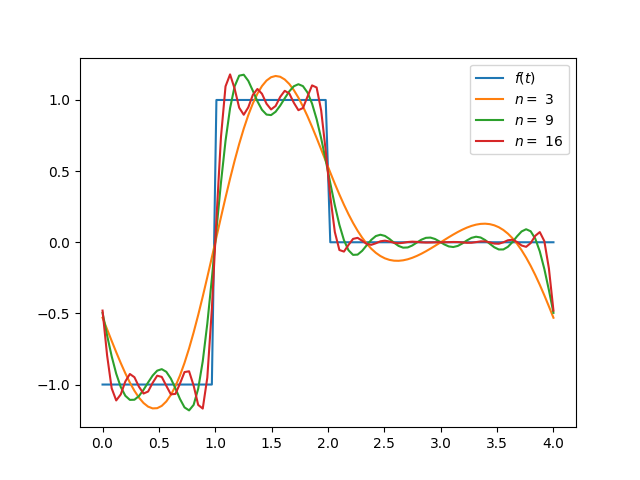
\includegraphics[width=0.95\textwidth]{figures/p2_synth.png}
    \end{center}
    \caption{Orignal and FOurier series representation of $f(t)$.}
\end{figure}
\clearpage

Here is some code that does it.

\begin{lstlisting}[language=python]
# imports
import numpy as np
import matplotlib.pyplot as plt


# original function
def func(t):
    out = np.zeros_like(t)
    out[t < 2] = 1.
    out[t < 1] = -1.

    return out

# our a_k series
def ak_fn(k):
    if k == 0:
        return 0.
    factor = np.exp(-1j * k * np.pi / 2) / (1j * np.pi * k)
    return factor * (1 - np.cos(k*np.pi / 2))

# synthesis eqn. for c.t. signals
def synth(t, n, ak_fn, period):
    out = np.zeros_like(t)
    for k in range(-n, n):
        out += np.real(ak_fn(k)*np.exp(1j * k * (2*np.pi / period) * t))
    return out

# create samples of times and functions values
ts = np.linspace(0, 4, 100)
fs = func(ts)

# make approximations for ifferent values of N
synths = {}
for k in [3, 9, 16]:
    synths[k] = synth(ts, k, ak_fn, 4)

# plot
fig, ax = plt.subplots()
ax.plot(ts, fs, label=r"$f(t)$")
for key in synths:
    ax.plot(ts, synths[key], label=f"$n = $ {key}")

ax.legend()
plt.savefig("figures/p2_synth.png")
plt.show()
\end{lstlisting}
